\phantomsection
\subsection{(10\%) Tạo và phân quyền cho thư mục \texttt{/data}}

Tạo thư mục \texttt{/data} trên server và phân quyền sao cho thành viên ban
giám đốc có toàn quyền (read, write và execute), các trưởng phòng có quyền read và
execute, các nhân viên không có bất cứ quyền gì. Ngoài ra chỉ chủ sở hữu tập tin có
quyền xóa hoặc đổi tên tập tin trong thư mục.


Để tạo và phân quyền cho thư mục \texttt{/data}, ta thực theo các bước như \textit{(\myref{fig:create-data-directory})}.

\begin{minipage}{.93\linewidth}
  \captionsetup{type=figure, skip=-15pt}
  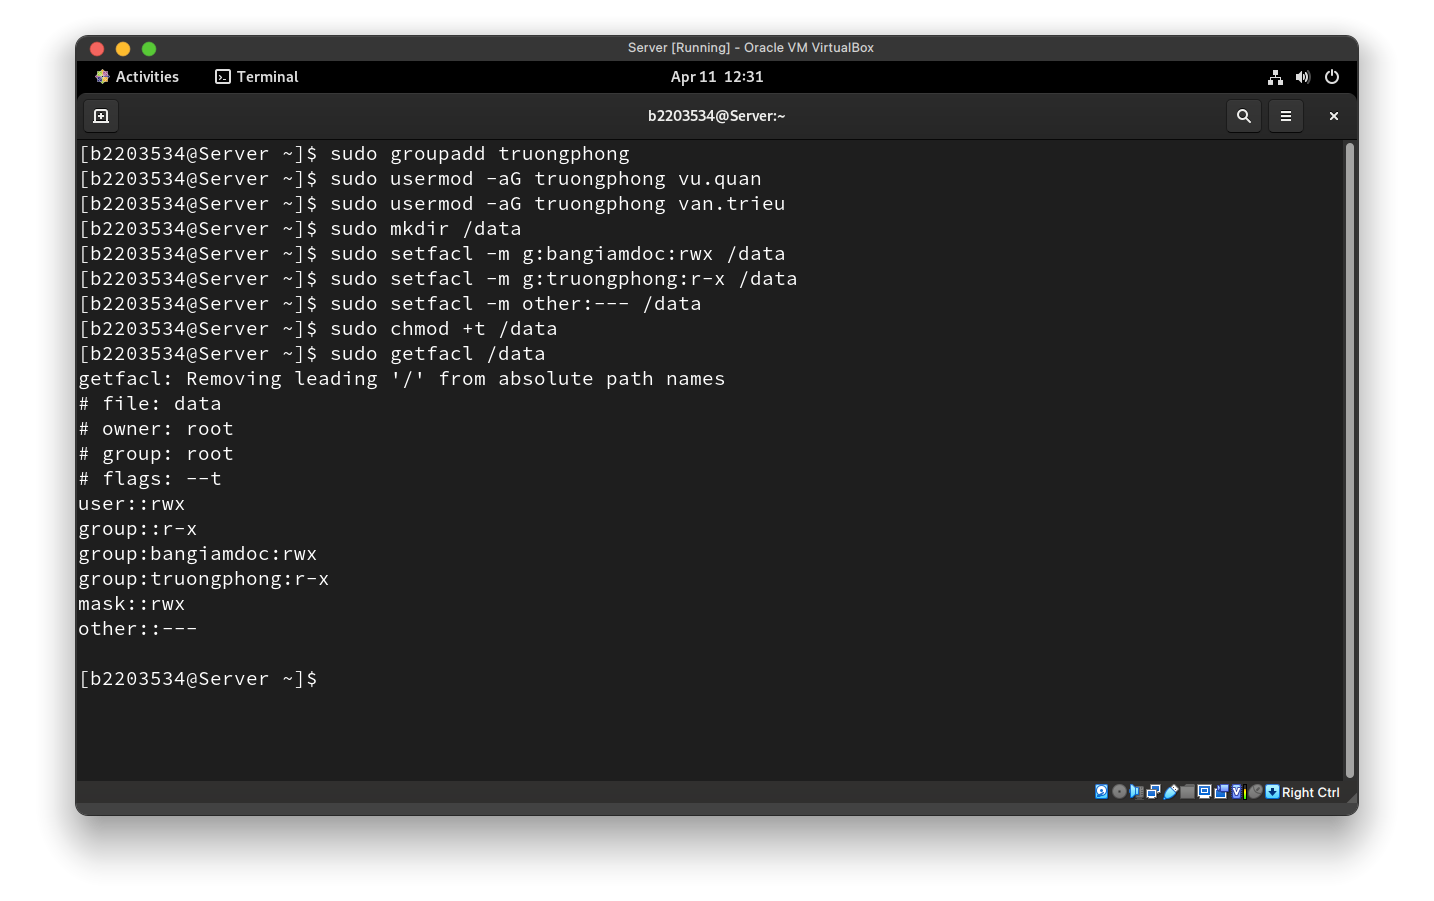
\includegraphics[width=\linewidth]{./imgs/Hinh-17.png}
  \caption{\bfseries Tạo và phân quyền cho thư mục \texttt{/data}}
  \label{fig:create-data-directory}
\end{minipage}

Cụ thể các bước như sau:

\begin{enumerate}
  \item Tạo nhóm \texttt{truongphong} và thêm người dùng vào.\\
        \begin{bashlisting}[gobble=10]{Tạo nhóm \texttt{truongphong} và thêm người dùng vào}
          sudo groupadd truongphong
          sudo usermod -aG truongphong vu.quan
          sudo usermod -aG truongphong phi.truong
        \end{bashlisting}
  \item Tạo thư mục \texttt{/data}.\\
        \begin{bashlisting}[gobble=10]{Tạo thư mục \texttt{/data}}
          sudo mkdir /data
        \end{bashlisting}
  \item Ban giám đốc có toàn quyền (read, write, execute) trên thư mục \texttt{/data}.\\
        \begin{bashlisting}[gobble=10]{Phân quyền cho ban giám đốc}
          sudo setfacl -m g:bangiamdoc:rwx /data
        \end{bashlisting}
  \item Trưởng phòng có quyền read và execute trên thư mục \texttt{/data}.\\
        \begin{bashlisting}[gobble=10]{Phân quyền cho trưởng phòng}
          sudo setfacl -m g:truongphong:r-x /data
        \end{bashlisting}
  \item Nhân viên không có bất cứ quyền gì trên thư mục \texttt{/data}.\\
        \begin{bashlisting}[gobble=10]{Phân quyền cho nhân viên}
          sudo setfacl -m other:--- /data
        \end{bashlisting}
  \item Chỉ chủ sở hữu tập tin có quyền xóa hoặc đổi tên tập tin trong thư mục \texttt{/data}.
        \begin{bashlisting}[gobble=10]{Phân quyền cho chủ sở hữu}
          sudo chmod +t /data
        \end{bashlisting}
\end{enumerate}
